% !TEX root = ../../main.tex
\section{Results}\label{sec:real_world_results}
In this section we will provide the results of our methods \gls{ocs-hats} applied to the real-world data sets and discuss the quality of the solution.
As stated above, we will use the quantitative quality metrics as used in \Cref{sec:artificial_data_quality_metrics}.
That will be in the form of a tabular overview of the (manually set) best meta-parameters and results, expressed in \gls{far} $\gamma$ and average delay $d_{avg}$ (following \Cref{sec:artificial_data_results}).
Furthermore, we have analyzed the results from an empirical point of view, since the problem of finding change points in human activities is ambiguous.
For the sake of brevity we excluded those observations from this chapter; they can be found in \Cref{AppendixA}.

\subsection{Quantitative metrics}
The employed two-stage algorithm requires the setting of user defined parameters.
In \Cref{tab:results_final_real_world} for each run the results are listed.
The right-most column summarizes the overall performance by taking the average over all the runs.
We have used a window length of 50 frames, which represents around $1.16$ seconds of data (the frame-rate of the recordings is not fixed).
The other parameter values, \ie the \gls{rbf} $\sigma$, high and low threshold, and proximity parameter $\delta$, are the result of an educated guess and manual optimization.
In general, a high value for the upper threshold and low value for the lower threshold indicates a robust method, since it indicates that change points are significantly different from homogeneous segments.
The chosen proximity $\delta$ should be low, since that indicates there will be few false positives.

To give a better impression on the quality of the $d_{avg}$, \Cref{fig:boxplot_final_real_world_runs} shows a box plot for each run.
It shows the spread of the $d_{avg}$ in seconds over all the change points.
A lower and more compact box plot is better.

\begin{table}[H]
  \centering
  \caption[Results real world runs]{Results of the real-world data sets. The used parameters are: window length = $50$, $\sigma = 13$, $th_{high} = 1.2$, $th_{low} = 0.8$, $\delta = 0.7$.
  The table shows the \gls{far} $\gamma$, average delay $d_{avg}$ and its spread, using the standard deviation.
  Low values are better.
  }
  \begin{tabulary}{\textwidth}{|l|c|c|c|c|c|c|c||c|}
    \cline{2-9}
    \multicolumn{1}{l|}{} & Run 1 & Run 2 & Run 3 & Run 4 & Run 5 & Run 6 & Run 7 & Average \\
    \hline
    $\gamma(Y)$ & 0.1 & 0.2 & 0.14 & 0.37 & 0.29 & 0.64 & 0.57 & 0.33 \\
    \hline
    $d_{avg}$ & 0.52 & 0.85 & 0.93 & 0.54 & 0.69 & 0.51 & 0.32 & 0.62\\
    \hline
    $std(d_{avg})$ & 0.71 & 0.31 & 0.68 & 0.37 & 0.50 & 0.44 & 0.35 & 0.48 \\
    \hline
  \end{tabulary}
  \label{tab:results_final_real_world}
\end{table}

\begin{figure}[H]
\centering
  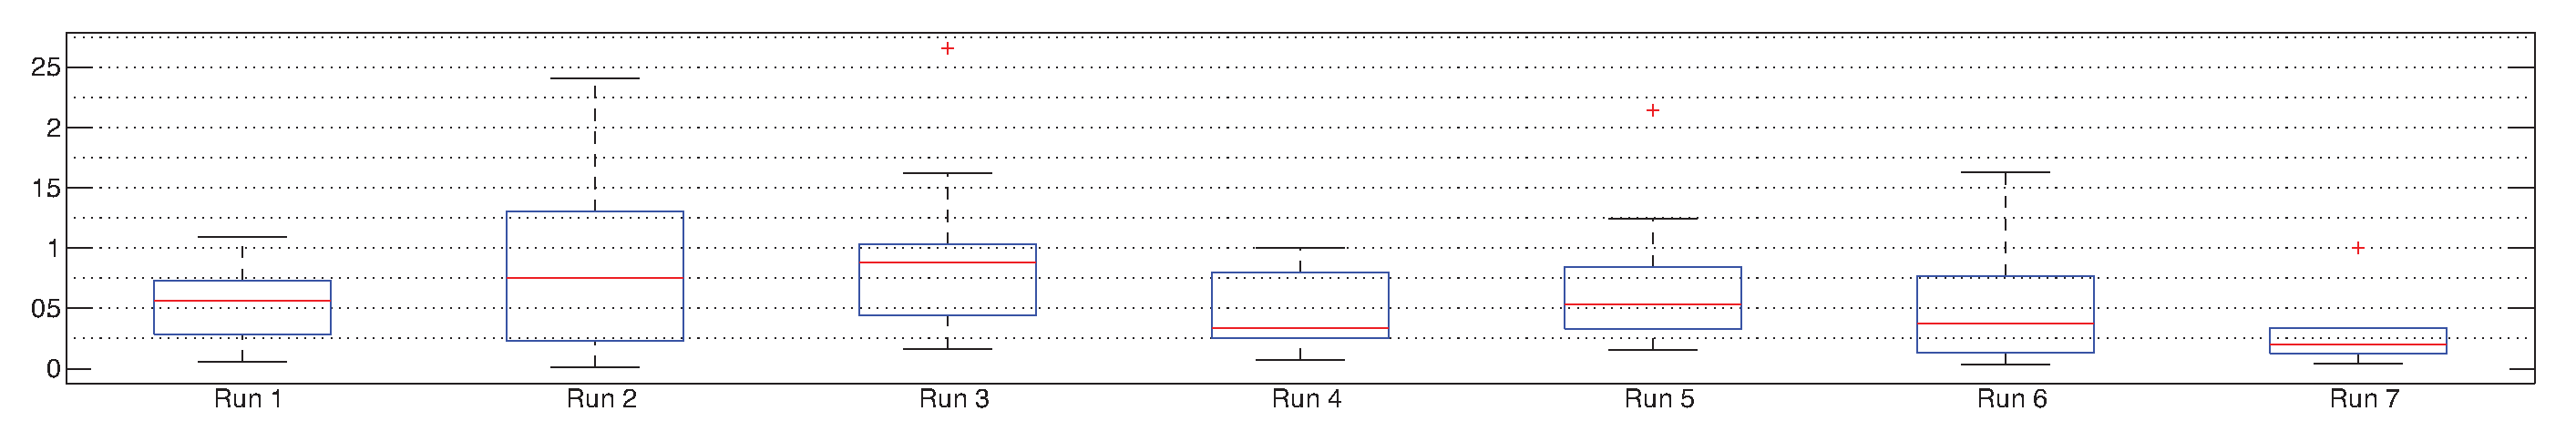
\includegraphics[width=1\textwidth]{./Figures/chapter6/data_collection/boxplot_final_runs.eps}
  \caption[Box plot results real-world runs]{Box plot of the results for the real-world runs, indicating the number of data points between the actual and closest detected change points. A lower and more compact box plot is better.}
  \label{fig:boxplot_final_real_world_runs}
\end{figure}

\subsection{Qualitative observations and remarks}\label{subsec:subjective_results}
It can be ambiguous where to place the (manually annotated) change points, in the case of real-world data.
The quantitative quality measure can give a distorted view on the performance.
To overcome this, we will state observations and remarks found after close (visual) inspection of the annotated and discovered change points.
In \Cref{fig:plots_all_runs_results} all the results are plotted.
The black solid lines indicate our manually determined change points.
The dashed purple lines indicate the change points as discovered by our method.
We will start with general observations applicable to all the runs.
A more detailed discussion for each run can be found in \Cref{AppendixA}.
Where possible, a graphical illustration will support our observations.

Overall our impression is that the proposed method is fairly good at recognizing change points.
Depending on the parameters for the sensitivity adjustment, almost all changes are discovered.

Our first observation is that with a high sensitivity it seems that the method produces many false positives.
Although the performed activity did not change around those false positives, there was a change in the recorded data.
This is a drawback of the method: since the sensitivity is set globally, it can produce false positive change points for some segments of a run.

The second observation is that the method often recognizes a change point \emph{before} our annotation.
Again, after closer inspection we can see that the data changes shape and distribution before we annotated a change based on the video recordings.
This effect can be observed in the case of a transition from running to walking; the last `steps' of running are already labeled as change points.
As with the above behavior, this is subject to parameter settings.

Considering the overall performance and results, we have the following observations:
\begin{itemize}
  \item \textbf{Merging:} in our method we use a proximity time period $\delta$ (usually up to $0.5$ - $1.0$ seconds) to merge discovered change points that are close together.
  Multiple merging-strategies can be applied, and in our method we use the naive implementation by simply ignoring all the discovered change points that occur less than $\delta$ seconds after the previous change point.
  This works well when there is a block of noisy data with a high amount of (falsely) discovered change points.
  On the flip side, this method will ignore real new change points which occur during the noisy period.
  This problem on itself can be formulated as a change detection problem.
  \item \textbf{Masking:} Since the parameters for the detection method are set globally, it is difficult to discover all the change points (and only the change points) without a high false alarm rate.
  If a change point is proceeded by a noisy block, then the real change point will be merged with the previous change points.
  In an other case, where a change point is very clear represented in the data but the next near change point is more subtle, the latter change point is \emph{masked} by the former.
  This masking effect is also discussed in \cite{inclan1994use}, where an iterated approach is applied.
  \item \textbf{Variance and threshold levels:} For our video synchronization, we started and ended each recording with a few seconds in which the recording smartphone was kept still in the air.
  Then we shake the smartphone to get a sudden change in the inertial sensor data, so the video and sensor data stream can easily be aligned.
  During the still period, the data variance, and thus the constructed hypersphere, becomes very small.
  As a results, even small movements are considered to be changes and in the case of a mid-air kept smartphone a lot of false change points are detected.
  Due to the merging effect described above, the final real change point (shaking the smartphone) is not discovered.
  \item \textbf{Incorrect weighting:} In our analyses we have used the data from the accelerometer, magnetic field, and rotation sensors.
  In the segments which embodied movement in a circular manner (such as walking and running around a fountain), the corner was not (or at a different time point) discovered.
  However, when we only used the magnetic field and rotation sensors, the corner was correctly discovered.
  Other transitions, such as from walking to running, are harder to discover without the (linear) accelerometer sensor data.
\end{itemize}

A more elaborate discussion with observations and remarks is provided in \Cref{AppendixA}.

\section{Possible improvements}\label{sec:possible_improvements}
From the above section we can extract a few possible improvements for the algorithm.
Most of the observations and remarks are due to a different required sensitivity for local segments of the run.
Currently, our method employs a global setting for the thresholds.
A possible improvement would be to use locally optimized parameters, although that would require an reflective data processing approach or more a priori information about the data.
The design decision for our approach was to create a general method, which requires no a priori knowledge about the data distribution.

Furthermore, we discovered that sometimes, especially with movements incorporating circular motions, the addition of (linear) accelerometer data makes the discovery of change points harder.
This problem can be handled by, for example, assigning weights to the sensor data streams.
Change can then be detected when it only occurs in one of the streams.